%!TEX TS-program = xelatex
%\documentclass[newPxFont]{beamer}
%\documentclass[newPxFont,handout]{beamer} % Раздаточный материал (на слайдах всё сразу)
\documentclass[aspectratio=169]{beamer} % Соотношение сторон


\usetheme{LTX}

%-=-=-=-=-=-=-=-=-=-=-=-=-=-=-=-=-=-=-=-=-=-=-=-=
%        LOADING PACKAGES
%-=-=-=-=-=-=-=-=-=-=-=-=-=-=-=-=-=-=-=-=-=-=-=-=
\usepackage{amsmath,amsfonts,amssymb,amsthm,mathtools}  % Тут мы подключаем пакеты для математики!
\usepackage{wasysym}
%%%%%%%%%%%%%%%%%%%%%%%% Шрифты %%%%%%%%%%%%%%%%%%%%%%%%%%%%%%%%%

\usepackage{fontspec}         % пакет для подгрузки шрифтов
\setmainfont{Helvetica}  % задаёт основной шрифт документа

% why do we need \newfontfamily:
% http://tex.stackexchange.com/questions/91507/
\newfontfamily{\cyrillicfonttt}{Helvetica}
\newfontfamily{\cyrillicfont}{Helvetica}
\newfontfamily{\cyrillicfontsf}{Helvetica}
% Иногда тех не видит структуры шрифтов. Эти трое бравых парней спасают ситуацию и доопределяют те куски, которые Тех не увидел.

% \usepackage{unicode-math}     % пакет для установки математического шрифта
% \setmathfont{Asana Math}      % шрифт для математики

\usepackage{polyglossia}      % Пакет, который позволяет подгружать русские буквы
\setdefaultlanguage{russian}  % Основной язык документа
\setotherlanguage{english}    % Второстепенный язык документа

%%% Работа с картинками
\usepackage{graphicx}  % Для вставки рисунков
\graphicspath{{images/}{images2/}}  % папки с картинками
\setlength\fboxsep{3pt} % Отступ рамки \fbox{} от рисунка
\setlength\fboxrule{1pt} % Толщина линий рамки \fbox{}
\usepackage{wrapfig} % Обтекание рисунков текстом

%%% Работа с таблицами
\usepackage{array,tabularx,tabulary,booktabs} % Дополнительная работа с таблицами
\usepackage{longtable}  % Длинные таблицы
\usepackage{multirow} % Слияние строк в таблице

%%% Программирование
\usepackage{etoolbox} % логические операторы

%%% Другие пакеты
\usepackage{multicol} % Несколько колонок

%%% Картинки
\usepackage{tikz} % Работа с графикой
\usepackage{pgfplots}
\usepackage{pgfplotstable}


\usepackage{xcolor}
\usepackage{hyperref}
\hypersetup{				
    unicode=true,           % позволяет использовать юникодные символы
    colorlinks=true,       	% true - цветные ссылки, false - ссылки в рамках
    urlcolor=blue,          % цвет ссылки на url
    linkcolor=red,          % внутренние ссылки
	hyperindex=true,        % сделать ли ссылку кликабельной?
	breaklinks=true         % если ссылка не умещается в одну строку, разбивать    
	                        % ли ее на две части?
}
\usepackage{verbatim}
\usepackage{fancyvrb}
\usepackage{mdframed}

 
\usepackage{chronology}

\renewcommand{\event}[3][e]{%
  \pgfmathsetlength\xstop{(#2-\theyearstart)*\unit}%
  \ifx #1e%
    \draw[fill=black,draw=none,opacity=0.5]%
      (\xstop, 0) circle (.2\unit)%
      node[opacity=1,rotate=45,right=.2\unit] {#3};%
  \else%
    \pgfmathsetlength\xstart{(#1-\theyearstart)*\unit}%
    \draw[fill=black,draw=none,opacity=0.5,rounded corners=.1\unit]%
      (\xstart,-.1\unit) rectangle%
      node[opacity=1,rotate=45,right=.2\unit] {#3} (\xstop,.1\unit);%
  \fi}%


\title{Уютный факультатив по \LaTeX}
\subtitle{Шрифты, документ в целом, преамбула для души}
\date{\today}

\begin{document}

\begingroup
\setbeamercolor{background canvas}{bg = LTXDarkGrey}
\begin{frame}[plain]
\centering  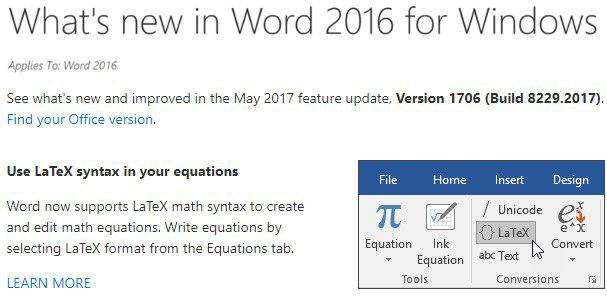
\includegraphics[width=0.95\linewidth]{new_word.jpg}	
\end{frame}
\endgroup 

\maketitle


\begin{frame}{Agenda} 
\begin{itemize}
	\item Снова увеличиваем интерактив!
	\item Графика в LaTeX, TikZ, Geogebra 
	\item Преамбула для души
	\item Душа за преамбулу 
\end{itemize}
\end{frame}


\section{TikZ} 

\section{Geogebra} 

\begin{frame}[plain]{Задание 1} 

\begin{enumerate}
	\item  Установить \alert{Geogebra 5}, нарисовать любую картинку
	\item  Экспортировать её в формате TikZ в \LaTeX
	\item  Центрировать его и оформить как картинку
	\item  Скачать какую-нибудь картинку из интернета
	\item  Сделать две картинки (из интернета и TikZ) рядом
\end{enumerate}

\begin{block}{Ссылка на Geogebra:}
	\vspace{3mm}
	\centerline {\url{ https://www.geogebra.org/download?lang=ru }}
	\vspace{3mm}
\end{block}
\end{frame}

\section{Показать cowsay} 

\section{Показать наклейки} 

\section{Преамбула для души} 

\section{Душа за преамбулу} 


\begin{frame}[plain]{Трасса 60}
\begin{center}

\includegraphics[width=0.95\linewidth]{road_60.png}	
\end{center}
\end{frame}


\begin{frame}
\begin{center}
	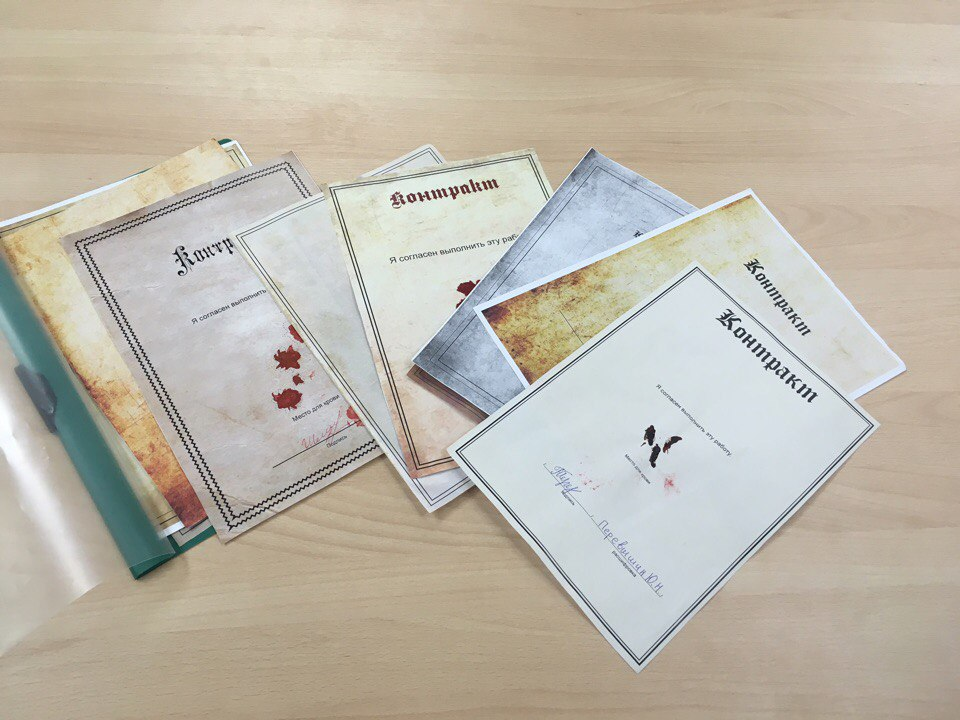
\includegraphics[width=0.8\linewidth]{contract_2.jpg}	
\end{center}
\end{frame}

\section{Свои команды и макросы} 


\begin{frame}[plain]{Задание 2} 

\begin{enumerate}
	\item Осталось время? Задавайте вопросы! 
	\item Уходите кушать 
	\item Либо начните делать домашку по оформлению письма из Хогвартса или послания. 
\end{enumerate}
\end{frame}



\begingroup
\setbeamercolor{background canvas}{bg = LTXDarkGrey}
\begin{frame}[plain]
\centering 
\includegraphics[width=0.7\linewidth]{arh.jpg}
\end{frame}
\endgroup 
\end{document}
